\documentclass[a4paper, twoside, english]{article}

\usepackage{amsmath}
\usepackage{amsfonts}
\usepackage{ihci}
\usepackage{graphicx}
\usepackage{subfig}

\graphicspath{{./../figures/}}

\title{Exercise 2 \\ 3D Computer Vision}  % Replace "Template Report" with Exercise 1, Exercise 2, etc
\author{Albert Garaev, Ksenia Novikova, Mukhammadsodik Khabibulloev }    % Replace with your names
\date{22.11.2021}                              % Replace with current date

\begin{document}

\maketitle

\section{Introduction}

This report presents the results of the theoretical and practical parts of Exercise 2.

\section{Theory}
\subsection{ Homography Definition}
The Homography is a projective transformation that transforms lines into lines (line preserving).  Homography is non-singular, invertible projective mapping $h:\ P^n \rightarrow P^n.$ 
Homography is represented by a $(n + 1)$-dimension square matrix with $(n + 1)^2 - 1$ degree of freedom (DOF) ~\cite{Stricker2021}.
\subsection{ Line Preservation}
Let $ x_1, x_2, x_3 \in P^2$ be three points on a line. We need to show that a non-singular matrix $H\in R^{3 \times 3}$ that
maps the points in projective space preserves this property.
At first, we need to calculate the homography matrix $H^{3 \times 3}$ ~\cite{Stricker2021}:

\begin{equation}
\begin{gathered}		
	\left(
	\begin{array}{ccc}
		x'_1\\
		x'_2\\
		x'_3
	\end{array}
	\right) = 
	\left[
	\begin{array}{ccc}
		h_{11}&h_{12}&h_{13}\\
		h_{21}&h_{22}&h_{23}\\
		h_{31}&h_{32}&h_{33}
	\end{array}
	\right]
	\left(
	\begin{array}{ccc}
		x_1\\
		x_2\\
		x_3
	\end{array}
	\right) 
	\label{eq:Homograph}
	\ or \ 
	x'=Hx \\ \leftrightarrow \\ 
	\lambda \left[
	\begin{array}{ccc}
		x'\\
		y'\\
		1
	\end{array}
	\right] = 
	\left[
	\begin{array}{ccc}
		h_{11}&h_{12}&h_{13}\\
		h_{21}&h_{22}&h_{23}\\
		h_{31}&h_{32}&h_{33}
	\end{array}
	\right]
	\left[
		\begin{array}{ccc}
		x\\
		y\\
		1
	\end{array}
	\right],
\end{gathered}	
\end{equation}
where $\lambda$ is constant scale factor. We use cross-product to remove this.
\begin{equation*}
	x'_i \times Hx_i= 0 \\ 
\end{equation*}
 Due to fact that only 2 equations linearly independent, we can remove third row:
 \begin{equation*}
 	x'_i \times Hx_i= 
 	\left[
 	\begin{array}{ccccccccc}
 		-x & -y & -1 & 0 & 0 & 0 & x'x &x'y & x'\\
 		0 & 0 & 0 & -x & -y & -1 & y'x & y'y & y'
 		
 	\end{array}
 	\right]  
 	\left[
 	\begin{array}{ccccccccc}
 		h_1 & h_2 & h_3 & h_4 & h_5 & h_6 & h_7 & h_8 & h_9 		
 	\end{array}
 	\right]\\ 
\end{equation*}
We can write  in matrix form:
 \begin{equation*}
 	A_ih=0,\ where \\
	A_i= 
	\left[
	\begin{array}{ccccccccc}
		-x & -y & -1 & 0 & 0 & 0 & x'x &x'y & x'\\
		0 & 0 & 0 & -x & -y & -1 & y'x & y'y & y'
		
	\end{array}
	\right]; \\ 
	h=\left[
	\begin{array}{c}
		h_1\\
		h_2\\
		h_3\\
		h_4\\
		h_5\\
		h_6\\
		h_7\\
		h_8\\
		h_9 		
	\end{array}
	\right]\\ 
\end{equation*}
We need for a minimal solution four matches (null space of 8x9 matrix). Four 2x9 $A_i$ matrices which can be used to get a single 8x9 matrix $A = [A_1\ A_2\ A_3\ A_4]^T$.

Definition of a line  can be represented by the following equation: ax+by+c = 0. Thus we can represent this line as the vector $(a,b,c)^T$. 
As we know, point $x_i$ lies on the line l if and only if $l^Tx_i = 0$. 
Let point x be on line l and point x' be on line l', then we have equations: $l^Tx = 0$ and $l'^Tx' = 0$
We get following equation using \ref{eq:Homograph}:
$l=H^Tl'$
Due to this fact we can represent the result below using homogeneous coordinates and equation \ref{eq:Homograph}:
\begin{equation*}
		\lambda \left[
	\begin{array}{ccc}
		x'\\
		y'\\
		1
	\end{array}
	\right] = 
	H^T
	\left[
	\begin{array}{ccc}
		x\\
		y\\
		1
	\end{array}
	\right],
\end{equation*}
where line l represented by $(x' \ y' \ 1)^T$. \\
Now we can calculate matrix $A_i$:
\begin{equation*}
	A_i= 
	\left[
	\begin{array}{ccccccccc}
		-x' & 0 & x'x & -y' & 0 & y'x & -1 & 0 & x\\
		0 & -x' & x'y & 0 & -y' & y'y & 0 & -1 & y
		
	\end{array}
	\right]	
\end{equation*}

We present the use of point and line matches. We get four 2x9 Ai matrices for each match $i$ which can be used to get a single 8x9 matrix $A$ and in turn this is the solution for the homography vector h.\\
Thereby, we have proved that the homography of H preserve the property of preserving the line, we show that both the points and the line can be invertibly mapped onto the projective plane.

\subsection{ Camera Center in Wold Coordinates}
$(a)$ We need to prove that the camera center in world coordinates $C_w$ can be expressed in terms of the extrinsic camera parameters by formula:\\
$C_w = -R^Tt$\\
A point in homogeneous world coordinates $C_w=(x_w,y_w,z_w)$ is transformed to camera coordinates $C_c=(x_c,y_c,z_c)$ to the formula below:\\
\begin{equation}
	\begin{gathered}
	\left(
	\begin{array}{ccc}
		x_c\\
		y_c\\
		z_c\\
		1
	\end{array}
	\right) =
	\left(
	\begin{array}{ccc}
		R & t\\
		0_{3}^T & 1
	\end{array}
	\right)
	\left(
	\begin{array}{ccc}
		x_w\\
		y_w\\
		z_w\\
		1
	\end{array}
	\right) \
	or\  C_c = [R| t]C_w\\
	\label{eq:matrixCW}
	\end{gathered}
\end{equation}

Using this equation we can present $C_w$:\\
$ C_w = [R| t]^{-1}C_c$\\
Camera center coordinate in camera coordinate system is $C_c=(0,0,0)$, so we need to find $[R| t]^{-1}$.
We calculate the formula for rotation matrix around all axis was found in Exercise 1:

\begin{equation*}
\begin{gathered}
	R= \left[
	\begin{array}{ccc}
		\cos\psi\cos\theta & -\sin\psi\cos\phi+\cos\psi\sin\theta\sin\phi & \sin\psi\sin\phi+\cos\psi\sin\theta\cos\phi\\
		\cos\theta\sin\psi & \cos\psi\cos\phi+\sin\theta\sin\psi\sin\phi  & -\cos\psi\sin\phi+\sin\theta\sin\psi\cos\phi\\
		-\sin\theta & \cos\theta\sin\phi & \cos\theta\cos\phi
	\end{array}
	\right] 
\end{gathered}
\end{equation*}

\begin{equation*}
	\begin{gathered}
		[R|t]= \left[
		\begin{array}{cccc}
			\cos\psi\cos\theta & -\sin\psi\cos\phi+\cos\psi\sin\theta\sin\phi & \sin\psi\sin\phi+\cos\psi\sin\theta\cos\phi & t_x\\
			\cos\theta\sin\psi & \cos\psi\cos\phi+\sin\theta\sin\psi\sin\phi  & -\cos\psi\sin\phi+\sin\theta\sin\psi\cos\phi & t_y\\
			-\sin\theta & \cos\theta\sin\phi & \cos\theta\cos\phi & t_z \\
			0&0&0&1
		\end{array}
		\right] 		
	\end{gathered}
\end{equation*}
As we know ${[R|t]^{-1}}={{{[R|t]^*}^T}\over{det[R|t]}}$\\
Let's find mitrix of algebraic complements $[R|t]^{*}$. We need to find the minor matrix M:\\
\tiny
\begin{equation*}
	\begin{gathered}
	M=\left[
\begin{array}{cccc}
	\cos\psi\cos\theta & \sin\psi\cos\phi-\cos\psi\sin\theta\sin\phi \\
	-\cos\theta\sin\psi & \cos\psi\cos\phi+\sin\theta\sin\psi\sin\phi \\
	-\sin\theta & -\cos\theta\sin\phi& \\
	t_x\cos\psi\cos\theta + t_y\cos\theta\sin\psi - t_z\sin\theta & t_x(\sin\psi\cos\phi-\cos\psi\sin\theta\sin\phi) -t_y(\cos\psi\cos\phi+\sin\theta\sin\psi\sin\phi) -t_z\cos\theta\sin\phi 
\end{array}
\right. \\
\left.
\begin{array}{cccc}
	 \sin\psi\sin\phi+\cos\psi\sin\theta\cos\phi & 0\\
	 \cos\psi\sin\phi-\sin\theta\sin\psi\cos\phi & 0\\
	 \cos\theta\cos\phi & 0\\
	 t_x(\sin\psi\sin\phi+\cos\psi\sin\theta\cos\phi)-t_y(\cos\psi\sin\phi-\sin\theta\sin\psi\cos\phi) + t_z\cos\theta\cos\phi&1
\end{array}
\right]
	\end{gathered}
\end{equation*}
\normalsize
Then the mitrix of algebraic complements $[R|t]^{*}$:
\tiny
\begin{equation*}
	\begin{gathered}
		M=\left[
		\begin{array}{cccc}
			\cos\psi\cos\theta & -\sin\psi\cos\phi+\cos\psi\sin\theta\sin\phi \\
			\cos\theta\sin\psi & \cos\psi\cos\phi+\sin\theta\sin\psi\sin\phi \\
			-\sin\theta & \cos\theta\sin\phi& \\
			-t_x\cos\psi\cos\theta - t_y\cos\theta\sin\psi + t_z\sin\theta & t_x(\sin\psi\cos\phi-\cos\psi\sin\theta\sin\phi) -t_y(\cos\psi\cos\phi+\sin\theta\sin\psi\sin\phi) -t_z\cos\theta\sin\phi 
		\end{array}
		\right. \\
		\left.
		\begin{array}{cccc}
			\sin\psi\sin\phi+\cos\psi\sin\theta\cos\phi & 0\\
			-\cos\psi\sin\phi+\sin\theta\sin\psi\cos\phi & 0\\
			\cos\theta\cos\phi & 0\\
			-t_x(\sin\psi\sin\phi+\cos\psi\sin\theta\cos\phi)+t_y(\cos\psi\sin\phi-\sin\theta\sin\psi\cos\phi) - t_z\cos\theta\cos\phi&1
		\end{array}
		\right]
	\end{gathered}
\end{equation*}
\normalsize
The determinant of the matrix is equal to 1, as it was proved earlier. Then ${[R|t]^{-1}}={{{[R|t]^*}^T}\over{det[R|t]}}$:\\
\tiny
\begin{equation*}
	\begin{gathered}
		[R|t]^{-1}={1\over 1}		
			\left[
		\begin{array}{cccc}
			\cos\psi\cos\theta & \cos\theta\sin\psi \\
			-\sin\psi\cos\phi+\cos\psi\sin\theta\sin\phi & \cos\psi\cos\phi+\sin\theta\sin\psi\sin\phi \\
			\sin\psi\sin\phi+\cos\psi\sin\theta\cos\phi & -\cos\psi\sin\phi+\sin\theta\sin\psi\cos\phi& \\
			0&0
		\end{array}
		\right. \\
		\left.
		\begin{array}{cccc}
			-\sin\theta & -t_x\cos\psi\cos\theta - t_y\cos\theta\sin\psi + t_z\sin\theta \\
			\cos\theta\sin\phi &  t_x(\sin\psi\cos\phi-\cos\psi\sin\theta\sin\phi) -t_y(\cos\psi\cos\phi+\sin\theta\sin\psi\sin\phi) -t_z\cos\theta\sin\phi\\
			\cos\theta\cos\phi & -t_x(\sin\psi\sin\phi+\cos\psi\sin\theta\cos\phi)+t_y(\cos\psi\sin\phi-\sin\theta\sin\psi\cos\phi) - t_z\cos\theta\cos\phi\\
			0&1
		\end{array}
		\right]
	\end{gathered}
\end{equation*}
\normalsize
Then due to homogeneous coordinates $ C_w = [R| t]^{-1}C_c$:\\
\begin{equation*}
\begin{gathered}	
C_w = [R| t]^{-1}(0 \ 0\ 0\ 1)^T=
\left[
\begin{array}{cccc}
	 -t_x\cos\psi\cos\theta - t_y\cos\theta\sin\psi + t_z\sin\theta \\
	t_x(\sin\psi\cos\phi-\cos\psi\sin\theta\sin\phi) -t_y(\cos\psi\cos\phi+\sin\theta\sin\psi\sin\phi) -t_z\cos\theta\sin\phi\\
	-t_x(\sin\psi\sin\phi+\cos\psi\sin\theta\cos\phi)+t_y(\cos\psi\sin\phi-\sin\theta\sin\psi\cos\phi) - t_z\cos\theta\cos\phi\\
	1
\end{array}
\right] =\\ =
\left(
\begin{array}{cc}
	R^T\\
	1
\end{array} 
\right)
\left(
 \begin{array}{cccc}
	-t_x\\
	-t_y\\
	-t_z\\
	1
\end{array} 
\right)= \text{(converting from homogeneous)} = R^T(-t)=-R^Tt
\end{gathered}
\end{equation*}
Thereby, we proved that the camera center in world coordinates $C_w$ can be expressed in terms of the extrinsic camera parameters by formula:\\
$C_w = -R^Tt$\\
$(b) $ We need to illustrate the meaning of $t = -RC_w $( i.e. from where to where does this vector point).
As it shown above $C_w = -R^Tt$, we can express t by multiplying this equation by R:\\
$C_wR = -R^TRt=Et=t$, thus $t = RC_w $.
However in this case, we can see that $t = (O_w,O_c)$ is translation vector between origins, where $O_w \ and \ O_c$ are center of world coordinate system center of camera coordinate system respectively. The elements of the translation matrix have the opposite sign (inverted).
\begin{figure}[h!]
	\centerline{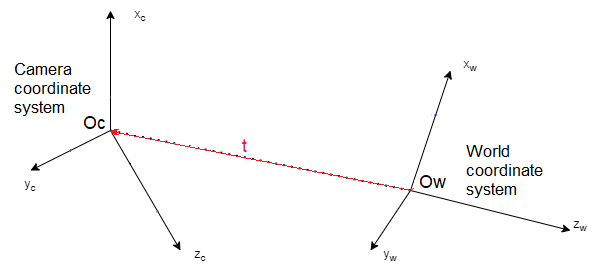
\includegraphics[width=0.55\textwidth]{trans.png}}
	\caption[trans]{ The meaning of translation vector in this context}
	\label{fig:trans}
\end{figure}
\section{Practical Part}
\subsection{Relative Rotation Estimation from Homography}
Why does the rotation matrix computed from H2 need correction?\\
Inverted matrix is not equal to transposed matrix and the determinant of this matrix is not equal to 1, i.e. the rotation matrix's properties are not fulfilled.
\subsection{Camera Pose Estimation from Homography}
The third element of t in part (a) above might be negative. What does this mean in this particular case (consider the location of the checkerboard corners)? Why can this happen?\\
The camera rotates in the opposite direction to the z-axis, when the third element of the vector t ($t_z$) is negative.





\bibliographystyle{plain}
\bibliography{bibliography.bib}
\end{document}